\documentclass[a4paper, 12pt]{article}

\usepackage[portuges]{babel}
\usepackage[utf8]{inputenc}
\usepackage[outline]{contour}
\usepackage[dvipsnames]{xcolor}
\usepackage{amsmath}
\usepackage{indentfirst}
\usepackage{graphicx}
\setlength{\jot}{8pt}
\usepackage[colorinlistoftodos]{todonotes}


\begin{document}

\begin{titlepage}
	\begin{center}
		\huge{Anotações sobre a Iniciação Científica}

		\vspace{30pt}
		
	\end{center}
	
	\begin{flushleft}
		%\begin{tabbing}
		%	Alunos\qquad\qquad\= \>Heitor Barroso Cavalcante - 12566101\\\\
		%	Professora\> Nina S. T. Hirata \\
		%
	    %\end{tabbing}
		Aluno\qquad\qquad Heitor Barroso Cavalcante - 12566101\\
		\vspace{10pt}
		Professora \quad Nina S. T. Hirata \\
		  
	\end{flushleft}
	\vspace{30pt}
	\begin{center}
		21 de Abril de 2022
	\end{center}
	\tableofcontents
\end{titlepage}
%%%%%%%%%%%%%%%%%%%%%%%%%%%%%%%%%%%%%%%%%%%%%%%%%%%%%%%%%%%\\
\thispagestyle{empty}

\newpage
\pagenumbering{arabic}

%%%%%%%%%%%%%%%%%%%%%%%%%%%%%%%%%%%%%%%%%%%%%%%%%%%%%%%%%
%%%%%%%%%%%%%%%%%%%%%%%%%%%%%%%%%%%%%%%%%%%%%%%%%%%%
\section{Processamento de Imagens Digitais}
\subsection{Introdução}
O processamento de imagens é uma subárea da disciplina de ``Processamento de Sinais", e essa subárea pode ser dividida em processamento digital ou analógico de imagens.
\begin{itemize}
    \item Processamento Analógico de Imagens:\\
    As imagens são manipuladas através da variação de sinais elétricos, o maior exemplo deste tipo de processamento é a imagem de televisão.
    \item Processamento Digital de Imagens:\\
    Consiste em desenvolver sistemas digitais para manipular imagens.
\end{itemize}

Nesse sentido, imagens podem ser compreendidas como um sinal bidimensional e pode ser definida como uma função \(f(x,y)\) tal que \((x,y)\) são as coordenadas de um pixel e \(f(x,y\) é o valor deste pixel. Assim, figuras visualizadas em um computador, por exemplo são matrizes de inteiros que variam de 0 a 255. As dimensões da imagem são as dimensões da matriz.
\\

Um sinal, pode ser definido como qualquer quantidade física medida através do tempo, do espaço ou qualquer outra dimensão. Logo, uma imagem digital pode ser caracterizada como um sinal de duas dimensões.
\\

A formação de uma imagem digital parte de um processo físico. A luz refletida pelos objetos fotografados é medida por diversos sensores e uma tensão contínua é gerada de acordo com a quantidade de luz captada pelos sensores. Agora, esse sinal analógico deve ser convertido para um digital. Para isso, amostragem e quantização são utilizadas para gerar a matriz de números que forma a imagem digital.
\\

Visão Computacional consiste no desenvolvimento de um sistema que consiga, a partir de uma imagem, gerar uma saída contendo informações sobre a imagem. Por exemplo, sistemas com reconhecimento facial.
\\

Por fim, resumindo, o processamento de sinais é muito importante para
o processamento de imagens. Sensores captam a luz do mundo físico, resultando em um sinal bidimensional que, após ser processado, forma uma imagem digital. Aí então esta imagem é manipulada através do processamento digital de imagens.

\subsection{Introdução à Sinais e Sistemas}
Primeiramente, definindo os termos chaves dessa seção:
\subsubsection{Sinais}
Em Engneharia elétrica, a medida fundamental para representação
de informações é chamada sinal. Um sinal poderia ter quaisquer dimensões
e ser de qualquer forma.
\begin{itemize}
	\item Sinais Analógicos:
    \\
	Um sinal analógico, medido através do tempo é um sinal contínuo.
	Eles são difíceis de analizar. Para representá-los, precisariamos de memória infinita.
	Isso ocorre pois a amostra é ``infinita''. Um exemplo é a voz humana ou $y = \sin(x)$.
	\item Sinais Digitais:
	\\
	São a apropriação dos sinais analógicos de uma maneira descontínua, valores discretos
	são utilizados para representar informações. Logicamente são menos precisos que sinais
	analógicos.
\end{itemize}
\subsubsection{Sistemas}
Um sistema é definido através dos tipos de sinais de entrada e dos tipos de sinais de saída
em relação aos quais o sistema funciona. Nesse caso, um sistema pode ser interpretado como o processo
de conversão de um sinal analógico para um sinal digital.
\\

Em tal tipo de conversão, há dois conceitos chave. Amostragem e Quantização.
Amostragem pode ser definido como o ato de tirar amostras do sinal isso ocorre no domínio da função que representa o sinal analógico.
Já Quantização pode ser definido como o ato de particionar os valores que a função pode assumir.


\section{Aplicações do Processamento de Imagens Digitais}
\begin{itemize}
	\item Restauração de imagens.
	\item Análise de imagens médicas.
  	\item Sensoriamento remoto.
   	\item Visão computacional.
    \item Reconhecimento de padrões.
    \item Processamento de vídeos.
    \item Análise de imagens microscópicas.
\end{itemize}

\section{Dimensões das Imagens}
Primeiramente, o conceito de dimensão define o número mínimo de pontos necessários para saber a posição de um objeto particular 
no espaço. No caso das imagens, sabemos que são bidimensionais. Altura e Largura. No caso de vídeos, podemos considerar o tempo como
 uma terceira dimensão e, por isso, podemos classificar esse tipo de imagens (vídeos) como 3D. Desso modo, podemos definir a imagem como
 uma função de duas variaveis.
 \begin{center}
	$f(x,y) = Imagem$
 \end{center}

 É interessante ressaltar que um filme pode ser considerado 3D. E, portanto, na realidade, um filme 3D seria 4D.

\section{Formação de Imagens em Câmeras}
Primeiro, é bom comentar sobre a formação de imagens no olho humano. A luz é refletida pelos objetos e é captada pelos olhos. Ao entrar no olho
a imagem fica invertida na retina. Então, o cérebro interpreta a imagem invertida e a ``desinverte''.
\subsection{Formação de Imagens em Câmeras Analógicas}
Nesse tipo de câmera, o filme --- uma tira plástica --- é revestida com halogeneto de prata. Essa substância reage com os fótons e forma
o negativo das imagens fotografadas.
\subsection{Formação de Imagens em Câmeras Digitais}
Nesse tipo de câmera, a formação das imagens se dá através do uso de um vetor de sensores CCD. CCD significa Charged Couple Devices.
Ou seja, dispositivo de carga acoplada, que é um sensor semicondutor que é sensível à imagem e a converte em um sinal elétrico. Há uma matriz
retangular desses sensores, em que cada um dos sensores corresponde à um pixel da imagem formada. Depois de cada sensor na matriz armazenar uma carga
a partir da incidência de fótons, tal carga é transformada em uma tensão que é convertida em informação digital. Isso ocorre em um sensor por vez.

\section{Mecanismos das Câmeras}
\subsection{Aperture - Abertura}
Como o próprio nome diz, é um orifício que permite a passagem da luz para dentro da câmera. Há lâminas que regulam o tamanho da abertura 
fazendo com que mais ou menos luz tenha acesso ao interior da câmera.
O efeito da abertura da câmera corresponde ao brilho da imagem fotografada
\subsection{Shutter - Obturador}
Podemos pensar no obturador como uma espécie de cortina que fica depois da abertura da câmera. Por trás do obturador está a matriz de 
dispositivos de carga acoplada. Assim que o obturador se abre a imagem é formada nessa matriz. Os efeitos do obturador dependem do tempo 
que a ele permanece aberto. Quanto mais tempo mais claridade haverá na imagem. Nesse sentido, dois conceitos chaves sobre esse mecanismo 
são o tempo e a velocidade. ``Shutter speed'' e ``Shutter time''. A velocidade representa quantas vezes o obturador se abriu ou se fechou, já o tempo 
representa o intervalo de tempo em que ele permanece aberto. É interessante ressaltar que há uma relação inversamente proporcional 
entre a velocidade e o tempo. Quanto mais velocidade, menor tempo e vice-versa. Uma aplicação importante da velocidade e do tempo do obturador é o ato de 
capturar imagens que se movimentam em alta velocidade. Assim, quanto menor for o tempo do obturador, melhor conseguiremos capturar imagens que se movem rapidamente.

\subsection{ISO}
O fator ISO representa a sensibilidade de uma câmera à luz. Quanto maior o número ISO de uma câmera, mais sensível ela é à luz. 
Contudo, há um sintoma colateral que se pronuncia quando o número ISO é elevado. Nesses casos, há mais ruído na imagem capturada.

\subsection{Conceito de Pixel}
O pixel é a unidade da imagem. Em uma imagem em gray-scale de 8 bits, cada pixel possui um valor de 0 a 255, que corresponde à intensidade 
da luz naquele ponto. Novamente, cada dispositivo de carga acoplada corresponde à um pixel.
\subsubsection{Cálculo do número total de pixels}
Para saber a quantidade de pixels em uma imagem, basta multiplicar as dimensões da matriz
\begin{center}
	$\#pixels = \#colunas \cdot \#linhas$
\end{center}
\subsubsection{Valores de pixels}
Sabemos que cada pixel possui somente um valor. Além disso, por definição, o valor $0$ significa ausência de luz.

\section{Transformação de Perspectiva}
De modo geral, um exemplo claro do que é perspectiva, é o fato de, através dos olhos humanos, ao vizualizar objetos menos distantes, 
esses aparentam ser maiores. Nesse sentido, a transformação de perspectiva é sobre a conversão de uma realidade tridimensional 
(altura, largura e profundidade) em um uma imagem bidimensional (altura e largura).

\subsection{Referencial - Frame of Reference}
\textcolor{red}{
	\large{ACHEI ESSA PARTE CONFUSA}
	\\
	Para analisar o mundo/imagem/cena tridimensional, precisamos de 5 referenciais --- ``frame of references'' --- sendo esses:
\begin{itemize}
	\item Objeto
	\item Mundo
 	\item Camera
 	\item Imagem
 	\item Pixel
\end{itemize}
}
\newpage
De qualquer maneira, essa transformação pode ser compreendida ao utilizarmos simpes conceitos de ótica e trigonometria. Observe:
\begin{figure}[!htbp]
	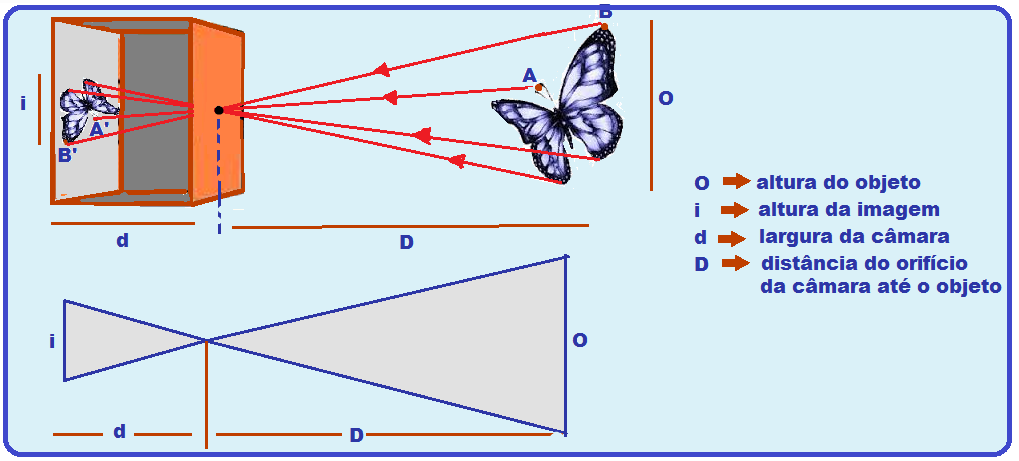
\includegraphics[scale=0.5]{images/otica.png}
	\caption{Imagem para exemplificar o uso da trigonometria na conversão do mundo 3D para o 2D}
\end{figure}
Podemos usar semelhança de triângulos para descobrir o tamanho da imagem formada $i$.
\begin{center}
	$\dfrac{i}{d} = \dfrac{O}{D} \Rightarrow i = d \dfrac{O}{D}$
\end{center}

\section{Conceito de bits por pixel}
O número de cores que podem ser representadas em uma imagem depende da quantidade de bits por pixel presente nessa imagem.
De maneira geral, podemos dizer que a maioria das imagens em gray-scale consiste de 8 bits por pixel. Equanto as coloridas tem, geralemente 
24 $bpp$. Isso pode ser compreendido ao imaginar que cada canal R, G, e B são possuem 8 bits.

Como dito anteriormente, o valor 0 é, por padrão, o valor que representa a cor preta, intensidade mínima em um canal de cor. 
Agora, o valor que representa o valor máximo não é padronizado, depende do $bbp$ dessa imagem. Então, teremos que esse valor pode ser 
representado por $2^{bpp} - 1$.

\subsection{Cálculo do tamanho (em memória) de uma imagem}
Para saber o tamanho de uma imagem, devemos levar em consideração as suas dimensões bidimensionais e o número de $bpp$. Por exemplo, digamos que 
uma imagem possua $1024$ linhas, $1024$ colunas e $8 bpp$, teremos:
\begin{center}
	$tamanho = 1024 \cdot 1024 \cdot 8 = 8388608 \; bits  \Rightarrow$ 
	\\
	\vspace*{0.15cm}
	$\Rightarrow tamanho = \dfrac{8388608}{8} = 1048576 \; bytes  \Rightarrow$ 
	\\
	$\Rightarrow tamanho = \dfrac{1048576}{1024} = 1024\;kb \Rightarrow tamanho = \dfrac{1024}{1024}\;Mb $
\end{center}

\section{Tipos de imagens}
\subsection{Imagem binária}
Nesse caso, há somente 2 valores possíveis para os pixels dessa imagem 0 ou 1. Onde 0 representa o preto e 1 o branco.
\begin{figure}[!htbp]
	\centering
	
\includegraphics[scale=0.5]{images/binaria.png}
	\caption{Imagem binária}
\end{figure}
\subsection{Formato 8 bits de cor}
Comumente conhecida como imagens Grayscale.
\begin{figure}[!htbp]
	\centering
	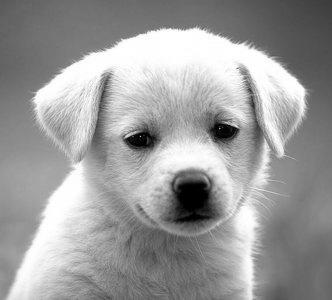
\includegraphics[scale=0.5]{images/grayscale.jpg}
	\caption{Imagem Grayscale}
\end{figure}

\subsection{Formato 16 bits de cor}
Aqui já temos imagens coloridas. Esses 16 bits são distribuídos nos 3 canais R, G e B. Da seguinte maneira:
\begin{itemize}
	\item 5 bits para o vermelho (R).
 \item 6 bits para o azul (G).
 \item 5 bits para o verde (B).
\end{itemize}

\subsection{Formato 24 bits de cor}
Por fim, temos o formato de imagens mais comuns hoje em dia. Em que temos esses 24 bits distribuídos igualmente entre os canais R, G e B.
\begin{figure}[!htbp]
	\centering
	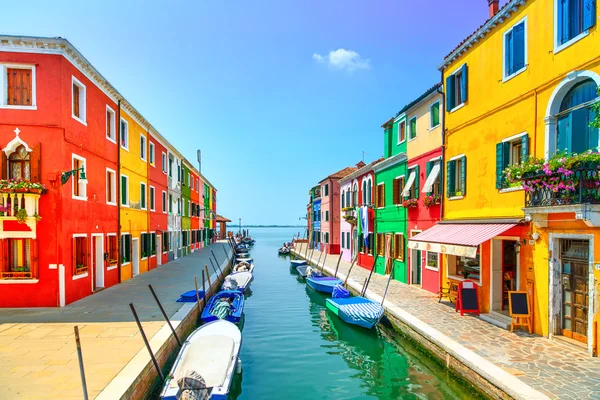
\includegraphics[scale=0.4]{images/colorida.png}
	\caption{Exemplo de imagem de 24 bits}
\end{figure}

\section{Códigos de cores}
Consideramos aqui que todas as cores estão no formato de 24bits. ou seja, uma cor ``$C$'' é tal que $(R, G, B) = (C_R, C_G, C_B)$
Assim, no formato RGB, temos:
\begin{itemize}
	\item \contour{black}{\textcolor{white}{Branco}} = (255, 255, 255)
 \item Preto = (0, 0, 0)
 \item \textcolor{red}{Vermelho} = (255, 0, 0)
 \item \textcolor{green}{Verde} = (0, 255, 0)
 \item \textcolor{blue}{Azul} = (0, 0, 255)
 \item \textcolor{gray}{Cinza} = (128, 128, 128)
		\\
		Nesse caso, a cor cinza é sempre o ponto médio entre a intensidade máxima e mínima. Logo, poderíamos escolher o valor 
		de 127 ou de 128. Nesse caso, escolhemos 128 (em todos os canais).
\end{itemize}

\subsection{Modelo CMYK}
Agora, vale ressaltar o modelo de cores CMYK --- comum em impressoras ---, aqui, CMYK significa ``cyan, magenta, yellow, black''. No conceito de impressoras,
geralmente há um cartucho de cores, (CMY) e outro preto. Assim, as cores ciano, magenta e amaerlo podem ser formadas ao se variar as porções de 
vermelho, verde e azul também. Os códigos RGB dessas cores são como segue.

\begin{itemize}
 \item \textcolor{magenta}{Magenta} = (255, 0, 255)
 \\
 Combinação de vermelho e azul.
 \item \textcolor{cyan}{Ciano} = (0, 255, 255)
 \\
 Combinação de verde e azul.
 \item \textcolor{yellow}{Amarelo} = (255, 255, 0)
 \\
 Uma combinação de vermelho e verde.
\end{itemize}

Além disso, também há o formato hexadecimal para representação de cores. Logo, para converter de um formato para outro, de RGB para hexadecimal ou 
vice versa, fazemos:

\subsection{Conversão RGB para Hexadecimal}
O formato de uma cor em hexadecimal é tal que \#FFFF00 (amarelo). para obter esses valores hexadecimais, deve-se, canal a canal RGB de uma dada cor, 
realizar a divisão do valor do canal por 16. Então, o quociente da divisão do canal R é o primeiro caracter do código, o segundo caracter 
é o resto dessa divisão. O terceiro valor é o quociente da divisão do valor do canal B por 16, o quarto é o resto dessa divisão. E assim por diante.
Observe:
\\
Sabemos que o código do \textcolor{yellow}{amarelo} é (255, 255, 0). Então, sobre R: $255/16$ tem quciente 15 e resto 15. FF. O mesmo ocorre com G. 
Agora, sobre B, teremos 00. Formando, assim o código \#FFFF00.

\subsection{Conversão Hexadecimal para RGB}
Para fazer o caminho inverso, devemos dividir o código hexadecimal em três porções. Sobre o exemplo do amarelo, temos FF, FF, 00. Agora, em um desses pares 
por vez, convertemos cada um de seus caracteres para binário. Concatenamos os dois números binários obtidos, convertemos para decimal e, assim, obtemos os valores dos canais. Observe: 
\\
Primeiramente, tratando de FF. convertendo para binário, temos 1111 e 1111. Concatenando: 11111111. Convertendo para decimal: 255 (valor do canal R)
Repetindo esses passos para os outros dois canais, obtemos o código da cor em (R, G, B).

\section{Conversão de RGB para Grayscale}
Primeiramente a maneira mais simples de se converter uma imagem para Grayscale é fazer a média entre os valores dos canais R, G e B.
\begin{figure}[!htb]
	\centering
	\minipage{0.30\textwidth}
	  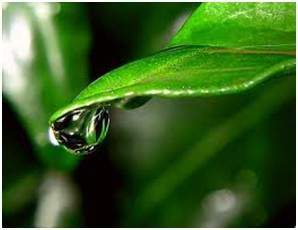
\includegraphics[width=\linewidth]{images/rgb.jpg}
	  \caption{Imagem original.}
	\endminipage\hspace{1cm}
	\minipage{0.30\textwidth}
	  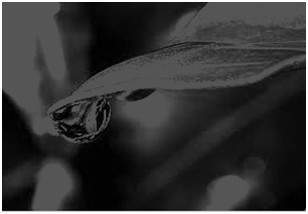
\includegraphics[width=\linewidth]{images/avg_gray.jpg}
	  \caption{Imagem Grayscale feita com a média}
	\endminipage
\end{figure}
Observe que essa figura não fica com um aspecto muito bom, fica ``empretecida''. Isso ocorre pois o olho humano não capta os níveis 
de vermelho, verde e azul na mesma proporção. Na realidade, o olho humano é muito mais sensível ao verde. Então, há o método de utilizar pesos para 
corrigir essas imperfeições. Então, se usarmos $30\%$ para o vermelho, $59\%$ para o verde e $11\%$ para o azul, teremos:

\begin{figure}[!htb]
	\centering
	\minipage{0.30\textwidth}
	  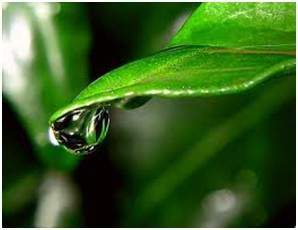
\includegraphics[width=\linewidth]{images/rgb.jpg}
	  \caption{Imagem original.}
	\endminipage\hspace{1cm}
	\minipage{0.30\textwidth}
	  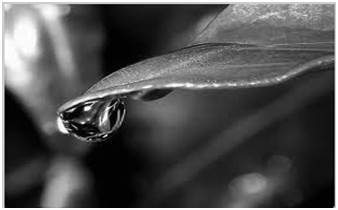
\includegraphics[width=\linewidth]{images/weighted_gray.jpg}
	  \caption{Imagem Grayscale feita utilizando pesos}
	\endminipage
\end{figure}


\section{Amostragem - Sampling}

Como dito anteriormente, o conceito de amostragem se relaciona ao processo de conversão de um sinal analógico para o digital. Assim, 
tiramos amostras do domínio da função que queremos converter. Logo, podemos correlacionar esse conceito com os pixels da imagem que será formada.
Imagine que queremos formar uma imagem de dimensões $5 \times 5$. Então, teremos que fazer uma amostragem da altura e largura do mundo que queremos representar 
em 5 valores diferentes cada. Ou seja, se a imagem é $f(x, y)$, $x$ assumirá 5 valores e $y$ assumirá 5 valores também. De maneira análoga, podemos 
relacionar esse conceito à matriz de dispositivos de carga acoplada ``CCDs''.

\subsection{Diferenças entre Zoom Analógico e Digital}
Apesar de ambos os conceitos se relacionarem ao fato de aumentarmos a amostragem do sinal, o zoom analógico aumenta essa amostragem através do movimento das lentes 
da câmera. Já o zoom digital funciona como se a imagem já houvesse sido capturada. Zoom analógico é feito nos sinais e o digital em uma imagem digital.

\section{Resolução de pixels}
De maneira simples, a resolução de uma imagem pode ser definida como a resolução a partir da qauntidade de pixels em uma imagem. Quando sabemos que a resolução de 
uma imagem é tal que $m \times n$ isso quer dizer que há $m$ colunas de pixel (largura) e $n$ linhas de pixel (altura). Nesse sentido, podemos calcular os 
MegaPixels de uma imagem fazendo $\dfrac{m \cdot n}{1\; mi}$ além disso, podemos saber o tamanho da imagem a partir de sua resolução também: 
$tamanho = pixelResolution \cdot bpp$ 

\subsection{Proporção da Tela}
Essa proporção nada mais é que a razão entre a largura da imagem e sua altura. Isso é extremamente útil ao mudar o tamnho das imagens, pois, 
se manetermos essa razão, então a imagem com tamanho modificado terá o mesmo aspecto que a imagem original.

\section{Mais sobre Zoom}
Como introduzimos os conceitos de zoom digital e analógico, podemos compará-los melhor. De fato, como o zoom analógico, ou óptico, nos proporciona 
um resultado melhor que o zoom digital. Isso ocorre pois, de fato estamos mudando a maneira como a fotografia será tirada, através do movimento das lentes.
Agora, o zoom digital, é simplesmente, aumentar uma certa área de vizualização de uma imagem, fazendo os pixels ficarem ``maiores''. Por isso, a qualidade da 
imagem é comprometida. Para fazer isso, há alguns métodos possíveis. ``Nearest neighbor interpolation'', ``Zero oeder hold method'', ``Zooming K times''.
\\

Um adendo interessante, é que o Exercício Programa 2 da disciplina de Laboratório de Métodos Numéricos, ministrada no primeiro semestre de 2022, tratou exatamente deste tópico.
Podemos considerar o ato de dar zoom em uma imagem com uma maneira de interpolar pontos, formando novos pixels a partir de pixels dados. Nesse sentido, estudamos os métodos de interpolação 
polinomial bilinear e bicúbica. Agora, continuemos a tratar dessas outras maneiras de dar zoom, que são abordadas no material.
\\

\subsection{Nearest Neighbor - Pixel Replication}
Para efetuar esse tipo de interpolação, devemos pensar, separadamente nas linhas e nas colunas da matriz que representa a imagem. Digamos que queremos 
aumentar a imagem por um fator de zoom $x$. Assim, assumindo que a imagem inicial tenha dimensões $3 \times 3$, por exemplo, e $x = 2$, a imagem final terá dimensões $6 \times 6$.
Agora, seja essa imagem exmplificada pela matriz:
\begin{table}[!htbp]
\centering
$
\begin{bmatrix}
	10 & 4 & 22 \\
	2 & 18 & 7 \\
	9 & 14 & 25
\end{bmatrix}
$
\end{table}

Primeiramente, devemos normalizar a posição dos pixels da nova imagem em relação à imagem antiga, fazemos isso sobre as linhas e sobre as colunas, obtendo uma razão entre 
o número de linhas da imagem original e o número de linhas da nova imagem. Análogo, para colunas. Então, obtemos duas proporções sobre as dimensões das duas imagens. 
Agora, múltiplicamos os índices de cada elemento da nova imagem por essa proporção. Desse modo, atribuiremos o valor do elemento (na imagem original) que possua índice mais próximo ao que 
foi calculado. Observe no exemplo, onde queremos interpolar os pontos $P_1$ e $P_2$.

$
\begin{bmatrix}
	10 & 4 & 22 \\
	2 & 18 & 7 \\
	9 & 14 & 25
\end{bmatrix}
\Rightarrow 
\begin{bmatrix}
	P_1 &  x &  x & x & x  & x \\
     x   &  x & x &  P_2 & x & x \\
	 x	& x & x &  x  &  x  & x  \\
	 x	& x & x &  x  &  x  & x \\
	 x	& x &  x  &  x  & x & x \\
	 x	& x & x &  x  &  x  & x \\
	 x	& x & x & x  & x  & x 

\end{bmatrix}$
Sabemos que a razão entre as linhas é: $\dfrac{3}{6} = \dfrac{1}{2}$ e as colunas a mesma. Então, o ponto $P_1$ tem coordenadas $(0, 0)$. 
Fazendo um produto escalar de $(0, 0)$ por $\left(\dfrac{1}{2}, \dfrac{1}{2}\right)$ teremos $(0, 0)$. O ponto $P_1$ tem ``vizinho mais próximo'' o pixel 
de coordenadas $(0, 0)$ na imagem original. $P_1 = 10$. Já em relação à $P_2$, teremos: $(1, 3) \cdot \left(\dfrac{1}{2}, \dfrac{1}{2}\right) = \left(0.5, 1.5\right)$. 
Tomando o teto: $(1, 2)$. O elemento $P_2$ tem vizinho mais próximo na imagem original o elemento de índice $(1, 2)$ e recebe seu valor. 
$P_2 = 7$. Fazendo o mesmo processo para todos os elementos, teremos a imagem com ``zoom'', ou seja, a imagem interpolada.
\begin{itemize}
\item Vantagem:
\\
É um processo extremamente simples.
\item Desvantagem:
\\
A imagem fica com um aspecto borrado.
\end{itemize}
Além disso, a imagem final terá tamanho tal que 
\\
$tamanhoFinal = \#linhasDaImagemOriginal \cdot fatorZoom \times \#colunasDaImagemOriginal \cdot fatorZoom$
\subsection{Zero-Order Hold - Bloqueio de Ordem Zero}
Esse algoritmo de zoom funciona de maneir muito simples. Para obter a imagem com zoom, devemos, colocar, entre os pixels da matriz da imagem original, 
pixels que tenham valores correspondentes à média dos seus vizinhos. Tome o exemplo:
\begin{center}
$
\begin{bmatrix}
1 & 2 \\
3 & 4
\end{bmatrix}
$
\end{center}
Inserindo uma linha entre as linhas dessa matriz, teremos:
\begin{table}
\centering
$
\begin{bmatrix}
1 & 1 & 2 \\
3 & 3 & 4
\end{bmatrix}
$
\end{table}

Observe que os valores insridos são o piso das médias obtidas. Agora, inserindo linhas entre as linhas:

\begin{table}
	\centering
	$
	\begin{bmatrix}
	1 & 1 & 2 \\
	2 & 2 & 3 \\
	3 & 3 & 4
	\end{bmatrix}
	$
\end{table}
Note que ocorreu o mesmo processo. A interpolação, ``zoom'' está feita.
\begin{itemize}
\item Vantagem:
\\
A imagem não fica com um aspecto borrado.
\item Desvantagem:
\\
Teremos que efeturar zoom nos baseando em potências de 2.
\end{itemize}

\subsection{K-times Zooming}
Esse algoritmo sana problemas dos que foram discutidos anteriormente. $K$ significa o fator de zoom.
Para explicar esse algoritmo, usaremos um exemplo. Tome a seguinte matriz como representação de uma imagem.
\begin{table}[!htbp]
	\centering
	$
	\begin{bmatrix}
	15 & 30 & 15 \\
	30 & 15 & 30
	\end{bmatrix}
	$
\end{table}
Primeiramente, supohemos $K = 3$. O número de valores que devem ser inseridos entre cada coluna e cada linha é $K - 1 = 3 - 1 = 2$.
Assim, iniciando pelas linhas (inserindo elementos entre as colunas) da matriz, temos que tomar os dois primeiros pixels 
adjacentes. ($15$ e $30$).
Subtraímos $15$ de $30$ ($15$). Dividimos o resultado da subtração por $K$ ($15/3 = 5$). Esse resultado é chamado de OP.
Agora devemos adicionar OP ao menor dos dois pixels escolhidos inicialmente ($5 + 15 = 20$) esse será o primeiro valor 
a ser inserido na matriz. Somamos OP a esse último resultado ($OP + 20 = 5 + 20 = 25$) e esse será o segundo elemento a ser
inserido na matriz, note que é o elemento de número $k - 1 = 2$ que foi inserido entre os dois primeiros elementos da primeira 
linha da matriz. Devemos fazer isso para todas as colunas. Ao fim desse processo, teremos a matriz:
\begin{table}[!htbp]
	\centering
	$
	\begin{bmatrix}
	15 & 20 & 25 & 30 & 20 & 25 & 15 \\
	30 & 20 & 25 & 15 & 20 & 25 & 30
	\end{bmatrix}
	$
\end{table}
\\
Depois de fazer isso, devemos ordenar os pixels inseridos de acordo com a ordem estaelecida na matriz. Por exemplo, no trecho:
$\begin{bmatrix}
	30 & \textcolor{blue}{20} & \textcolor{blue}{25} & 15	
\end{bmatrix}
$
\\
Tivemos os elementos em \textcolor{blue}{azul} inseridos. Note que a ordem da matriz era decrescente, da esquerda para a direita, indo 
de $30$ indo até $15$. Então, ordenaremos $\textcolor{blue}{20}$ e $\textcolor{blue}{25}$ em ordem decrescente também. Desse modo, 
Obteremos a seguinte matriz:
\begin{table}[!htbp]
	\centering
	$
	\begin{bmatrix}
	15 & 20 & 25 & 30 & 25 & 20 & 15 \\
	30 & 25 & 20 & 15 & 20 & 25 & 30
	\end{bmatrix}
	$
\end{table}
\\

Agora, precisamos efetuar o mesmo processo entre as linhas da matriz. Teremos:
\begin{table}[!htbp]
	\centering
	$
	\begin{bmatrix}
		15 & 20 & 25 & 30 & 25 & 20 & 15 \\
		20 & 21 & 21 & 20 & 21 & 21 & 20 \\
		25 & 22 & 22 & 25 & 22 & 22 & 25 \\
		30 & 25 & 20 & 15 & 20 & 25 & 30
	\end{bmatrix}
	$
\end{table}
Observe que usamos o piso da divisão de $5$ por $3$, e obtemos OP igual a $1$.

\large{\textcolor{red}{FIQUEI CONFUSO AQUI. O TUTORIAL DIZ QUE A IMAGEM FINAL FICA ASSIM, MAS EU NÃO TERIA QUE ORDENAR OS ELEMENTOS 
QUE FORAM INSERIDOS NOVAMENTE?}}

As dimensões da imagem final serão: $(K(\#linhas - 1) + 1) \times (K(\#colunas - 1) + 1)$

\begin{itemize}
	\item Vantagens:
 	\\
	Esse algoritmo combina as qualidades dos dois msotrados anteriormente. Não temos restrições quanto às dimensões da imagem final 
	e a imagem não fica muito borrada.
	\item Desvantagens:
 	\\
	Devido à necessidade de ordenação, esse algoritmo fica computacionamente mais custoso que os demais.
\end{itemize}

\section{Resolução Espacial - Spatial Resolution}
Esse tipo de resolução se relaciona ao menor detalhe que pode ser identificado em uma imagem. Podemos definir essa resolução também como 
o número de pixels independentes por polegada. Em suma, esse conceito se refere à comparação de imagens de uma mesma resolução (mesmas 
dimensões) para saber qual possui mais nitidez. Observe:
\begin{figure}[!htb]
	\centering
	\minipage{0.30\textwidth}
	  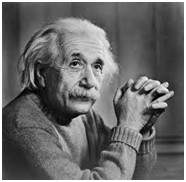
\includegraphics[width=\linewidth]{images/einsteinNitido.jpg}
	  \caption{Imagem com maior resolução espacial}
	\endminipage\hspace{1cm}
	\minipage{0.30\textwidth}
	  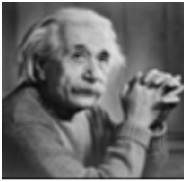
\includegraphics[width=\linewidth]{images/einstein_spatial.jpg}
	  \caption{Imagem com menor resolução espacial}
	\endminipage
\end{figure}
Podemos medir esse tipo de resolução das seguintes maneiras:
\begin{itemize}
	\item Pontos por Polegada.
 	\item Pixels por Polegada.
\end{itemize}

\subsection{Pixels por Polegada}
Geralmente usada para medir qualidade de telas, sabemos que, para obter essa unidade, devemos, primeiramente, 
obter a diagonal em pixels do visor calculada, a partir de sua resolução em pixels. $c = \sqrt[]{altura^2 + largura^2}$
Depois disso, dividiremos essa diagonal em pixels pelo tamanho da diagonal. $PPi = c/diagonalPolegadas$.

\subsection{Pontos por Polegada}
Essa unidade é, geralmente, utilizada para representar a qualidade de impressoras. Isto é, mede quantos pontos de tinta são impressos 
por polegada.

\section{Resolução Grayscale}
Resgatando conceitos já tratados anteriormente, a resolução em Grayscale tem íntima relação com a medida de $bpp$ (bits por pixel). Ou seja, 
quanto mais nuances de cinza puderem ser representadas, maior a resolução dessa imagem em termos de grayscale. Ainda, o total de nuances de cinza 
que podem ser exibidas nessa imagem com $bpp = k$ é tal que $2^k$, mas podemos também representar essa resolução puramente pelo número de 
$bpp$ e não pela quantidade de nuances de cinza que esse número produz.

\section{Conceito de Quantização}
Já sabemos que, no processo de conversão de um sinal analógico para um digital, há os conceitos de amostragem e quantização. Amostragem é 
feita no domínio do sinal, ou função. Já a quantização, é realizada nos valores que a função pode assumir. Ou seja, na imagem dessa função, feita no eixo 
$y$. Na realidade, ao quantizar um sinal, estamos digitalizando as amplitudes desse sinal, as particionando. Nesse sentido, podemos interpretar a resolução 
grayscale de uma imagem como um exemplo de quantização. Ao limitar os valores de cor que a imagem pode assumir, estamos quantizando as amplitudes do sinal.
Então, observe as diferenças entre Imagens com diferentes níveis de resolução grayscale (quantizações distintas).
\begin{figure}[!htb]
	\centering
	\minipage{0.17\textwidth}
	  	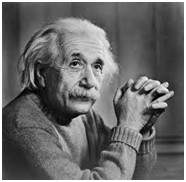
\includegraphics[width=\linewidth]{images/einstein256.jpg}
	  	\caption{256 níveis de cinza.}
	\endminipage\hspace{1cm}
	\minipage{0.17\textwidth}
	 	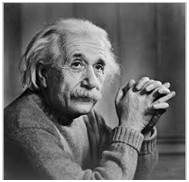
\includegraphics[width=\linewidth]{images/128.jpg}
	  	\caption{128 níveis de cinza.}
	\endminipage\hspace{1cm}
	\minipage{0.17\textwidth}
		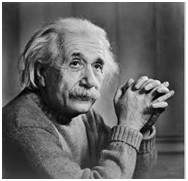
\includegraphics[width=\linewidth]{images/64.jpg}
		\caption{64 níveis de cinza.}
  	\endminipage\hspace{1cm}
  	\minipage{0.17\textwidth}
  		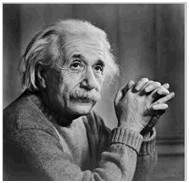
\includegraphics[width=\linewidth]{images/32.jpg}
  		\caption{32 níveis de cinza.}
	\endminipage
\end{figure}
\\
\begin{figure}[!htb]
	\centering
	\minipage{0.17\textwidth}
	  	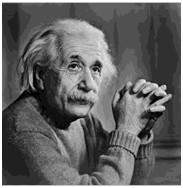
\includegraphics[width=\linewidth]{images/16.jpg}
	  	\caption{16 níveis de cinza.}
	\endminipage\hspace{1cm}
	\minipage{0.17\textwidth}
	 	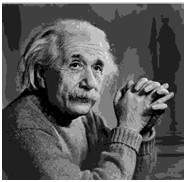
\includegraphics[width=\linewidth]{images/8.jpg}
	  	\caption{8 níveis de cinza.}
	\endminipage\hspace{1cm}
	\minipage{0.17\textwidth}
		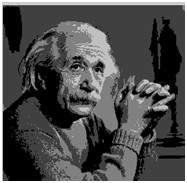
\includegraphics[width=\linewidth]{images/4.jpg}
		\caption{4 níveis de cinza.}
  	\endminipage\hspace{1cm}
  	\minipage{0.17\textwidth}
  		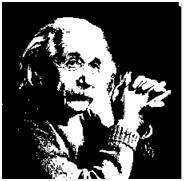
\includegraphics[width=\linewidth]{images/2.jpg}
  		\caption{ níveis de cinza.}
	\endminipage
\end{figure}

\section{Curvas de Preferência ISO - ISO Preference curves}
Como podemos observar nas imagens acima, a partir de uma certa quantidade de níveis de cinza, há o aparecimento de linhas na imagem. 
Tais linhas são chamadas de ``countouring''. Note que quanto mais discretizarmos (maior quantização) a imagem, mais aparecem essas linhas.
Contudo, esse não é o único fator que influencia no ``countouring''.
\subsection{Curvas de Isopreferência}
Em suma, estudos comprovaram que o aparecimento das linhas características do ``countouring'' está também relacionado à quantidade de detalhes presentes 
na imagem. Isso quer dizer que quanto mais detalhes uma imagem tiver, mais demorará para o efeito do ``countouring'' se tornar evidente.

\section{Conceito de Dithering \textcolor{red}{ACHEI ESSA SEÇÃO CONFUSA}}
Dithering é uma forma de ruído digital aplicado intensionalmente em um sinal. Nesse sentido, podemos ``permutar'' os pixels de uma imagem com baixos níveis de grayscale 
utilizando dithering para tornar mais detalhes visíveis nessa imagem.
\\

Primeiro, devemos trabalhar com limiares --- thresholding --- 

\section{Introdução a Histogramas}
\subsection{Histograma de uma Imagem}
O histograma de uma imagem mostra as frequências das intensidades dos pixels. Tomando, novamente, o exemplo de uma imagem grayscale, no eixo $x$, teremos 
as intensidades (níveis) de cinza presentes na imagem, enquanto no eixo $y$, teremos a frequência de ocorrência dessas intensidades.
\\
\begin{figure}[!htb]
	\centering
	\minipage{0.30\textwidth}
	  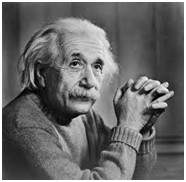
\includegraphics[width=\linewidth]{images/einsteinNitido.jpg}
	  \caption{Imagem}
	\endminipage\hspace{1cm}
	\minipage{0.30\textwidth}
	  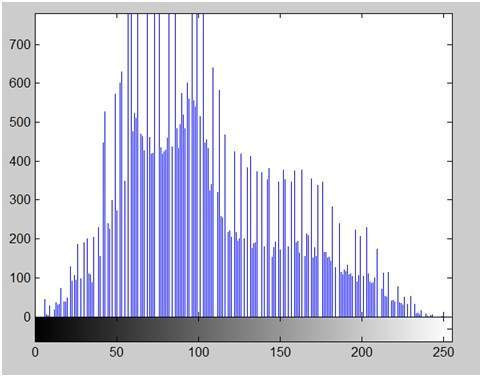
\includegraphics[scale=0.3]{images/histograma.jpg}
	  \caption{Histograma da Imagem}
	\endminipage
\end{figure}
\subsection{Aplicações dos Histogramas}
Uma das principais utilidades dos histogramas é a análise geral de imagens, podemos examinar uma imagem a partir de seu histograma. Além disso, 
estudar o brilho e contraste da imagem pode ser feito através do histograma. Por fim, há amplos usos em limiar --- thresholding ---, que são utilizados 
em visão computacional.
\end{document}






